\chapter{Resultados}
\label{cap:resultados}

Neste capítulo, são apresentados os resultados da compressão de imagens \acrshort{DICOM} dos órgãos pulmão, mama e cérebro utilizando os algoritmos \acrshort{PNG}, \acrshort{JPEG} e \acrshort{PCA} (com diferentes níveis de variância explicada). Inicialmente, é feita uma análise qualitativa com comparações visuais entre uma imagem original e suas versões comprimidas. Em seguida, são apresentadas as análises quantitativas das taxas de compressão e da qualidade aparente (\acrshort{PSNR}), agrupadas por algoritmo e tipo de órgão.

\section{Comparação Visual das Imagens}

Nas Figuras~\ref{fig:comparacao_pulmao}, \ref{fig:comparacao_mama} e \ref{fig:comparacao_cerebro}, são apresentadas as comparações visuais entre as imagens originais e suas versões comprimidas por cada método. Essas comparações permitem observar o impacto visual de cada método de compressão, considerando diferentes tipos de órgãos.

\begin{itemize}
    \item \textbf{Pulmão:} Na Figura~\ref{fig:comparacao_pulmao}, é apresentada a comparação visual das imagens de pulmão. Essas imagens possuem áreas homogêneas que favorecem altas taxas de compressão em todos os métodos, resultando em perdas visuais mínimas mesmo em cenários de maior redução, como no \acrshort{JPEG} e no \acrshort{PCA}.
    \begin{figure}[H]
        \centering
        \UNIFORfig{
            \Caption{\label{fig:comparacao_pulmao} Comparação visual das imagens de pulmão: original e comprimidas por \acrshort{PNG}, \acrshort{JPEG} e \acrshort{PCA}.}
        }{
            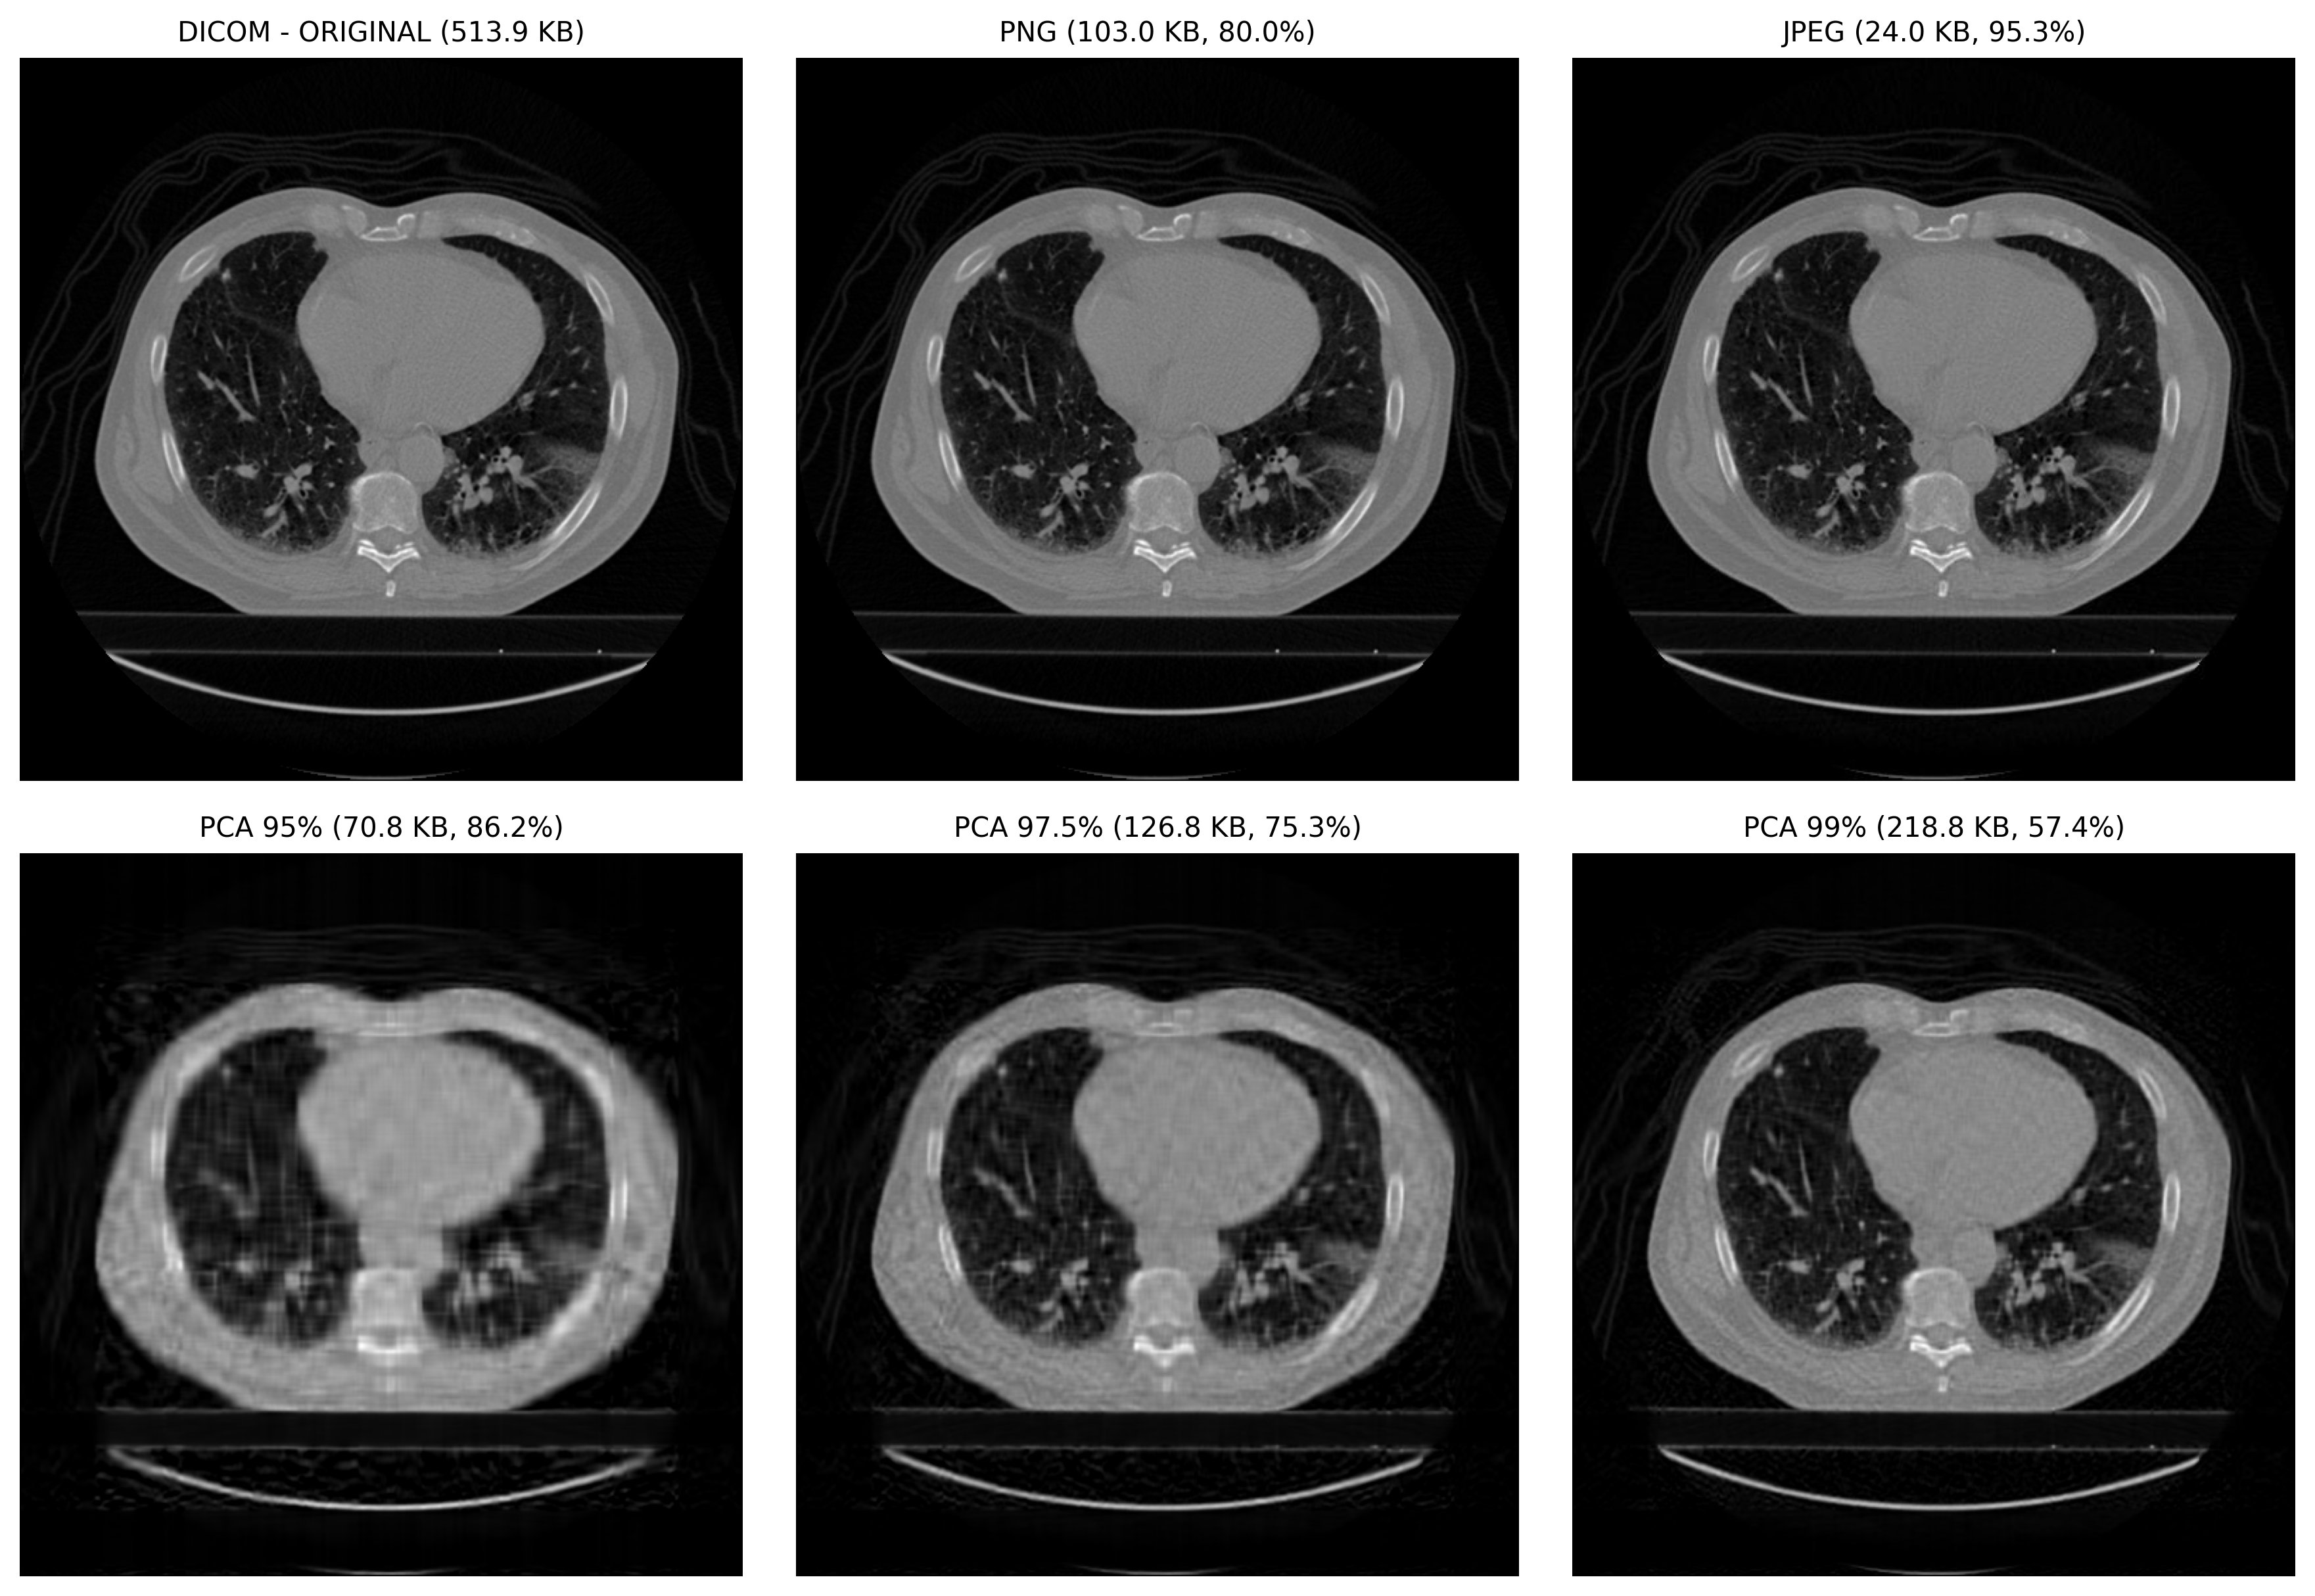
\includegraphics[width=\textwidth]{images/result-lung.png}
        }{
            \Fonte{Elaborado pelo autor.}
        }	
    \end{figure}
    \item \textbf{Mama:} A Figura~\ref{fig:comparacao_mama} apresenta as imagens de mama, que possuem alta densidade de detalhes. Essa característica dificultou a compressão, especialmente em cenários de maior redução, como o \acrshort{PCA} em 95\%, resultando em perdas mais perceptíveis visualmente.
    \begin{figure}[H]
        \centering
        \UNIFORfig{
            \Caption{\label{fig:comparacao_mama} Comparação visual das imagens de mama: original e comprimidas por \acrshort{PNG}, \acrshort{JPEG} e \acrshort{PCA}.}
        }{
            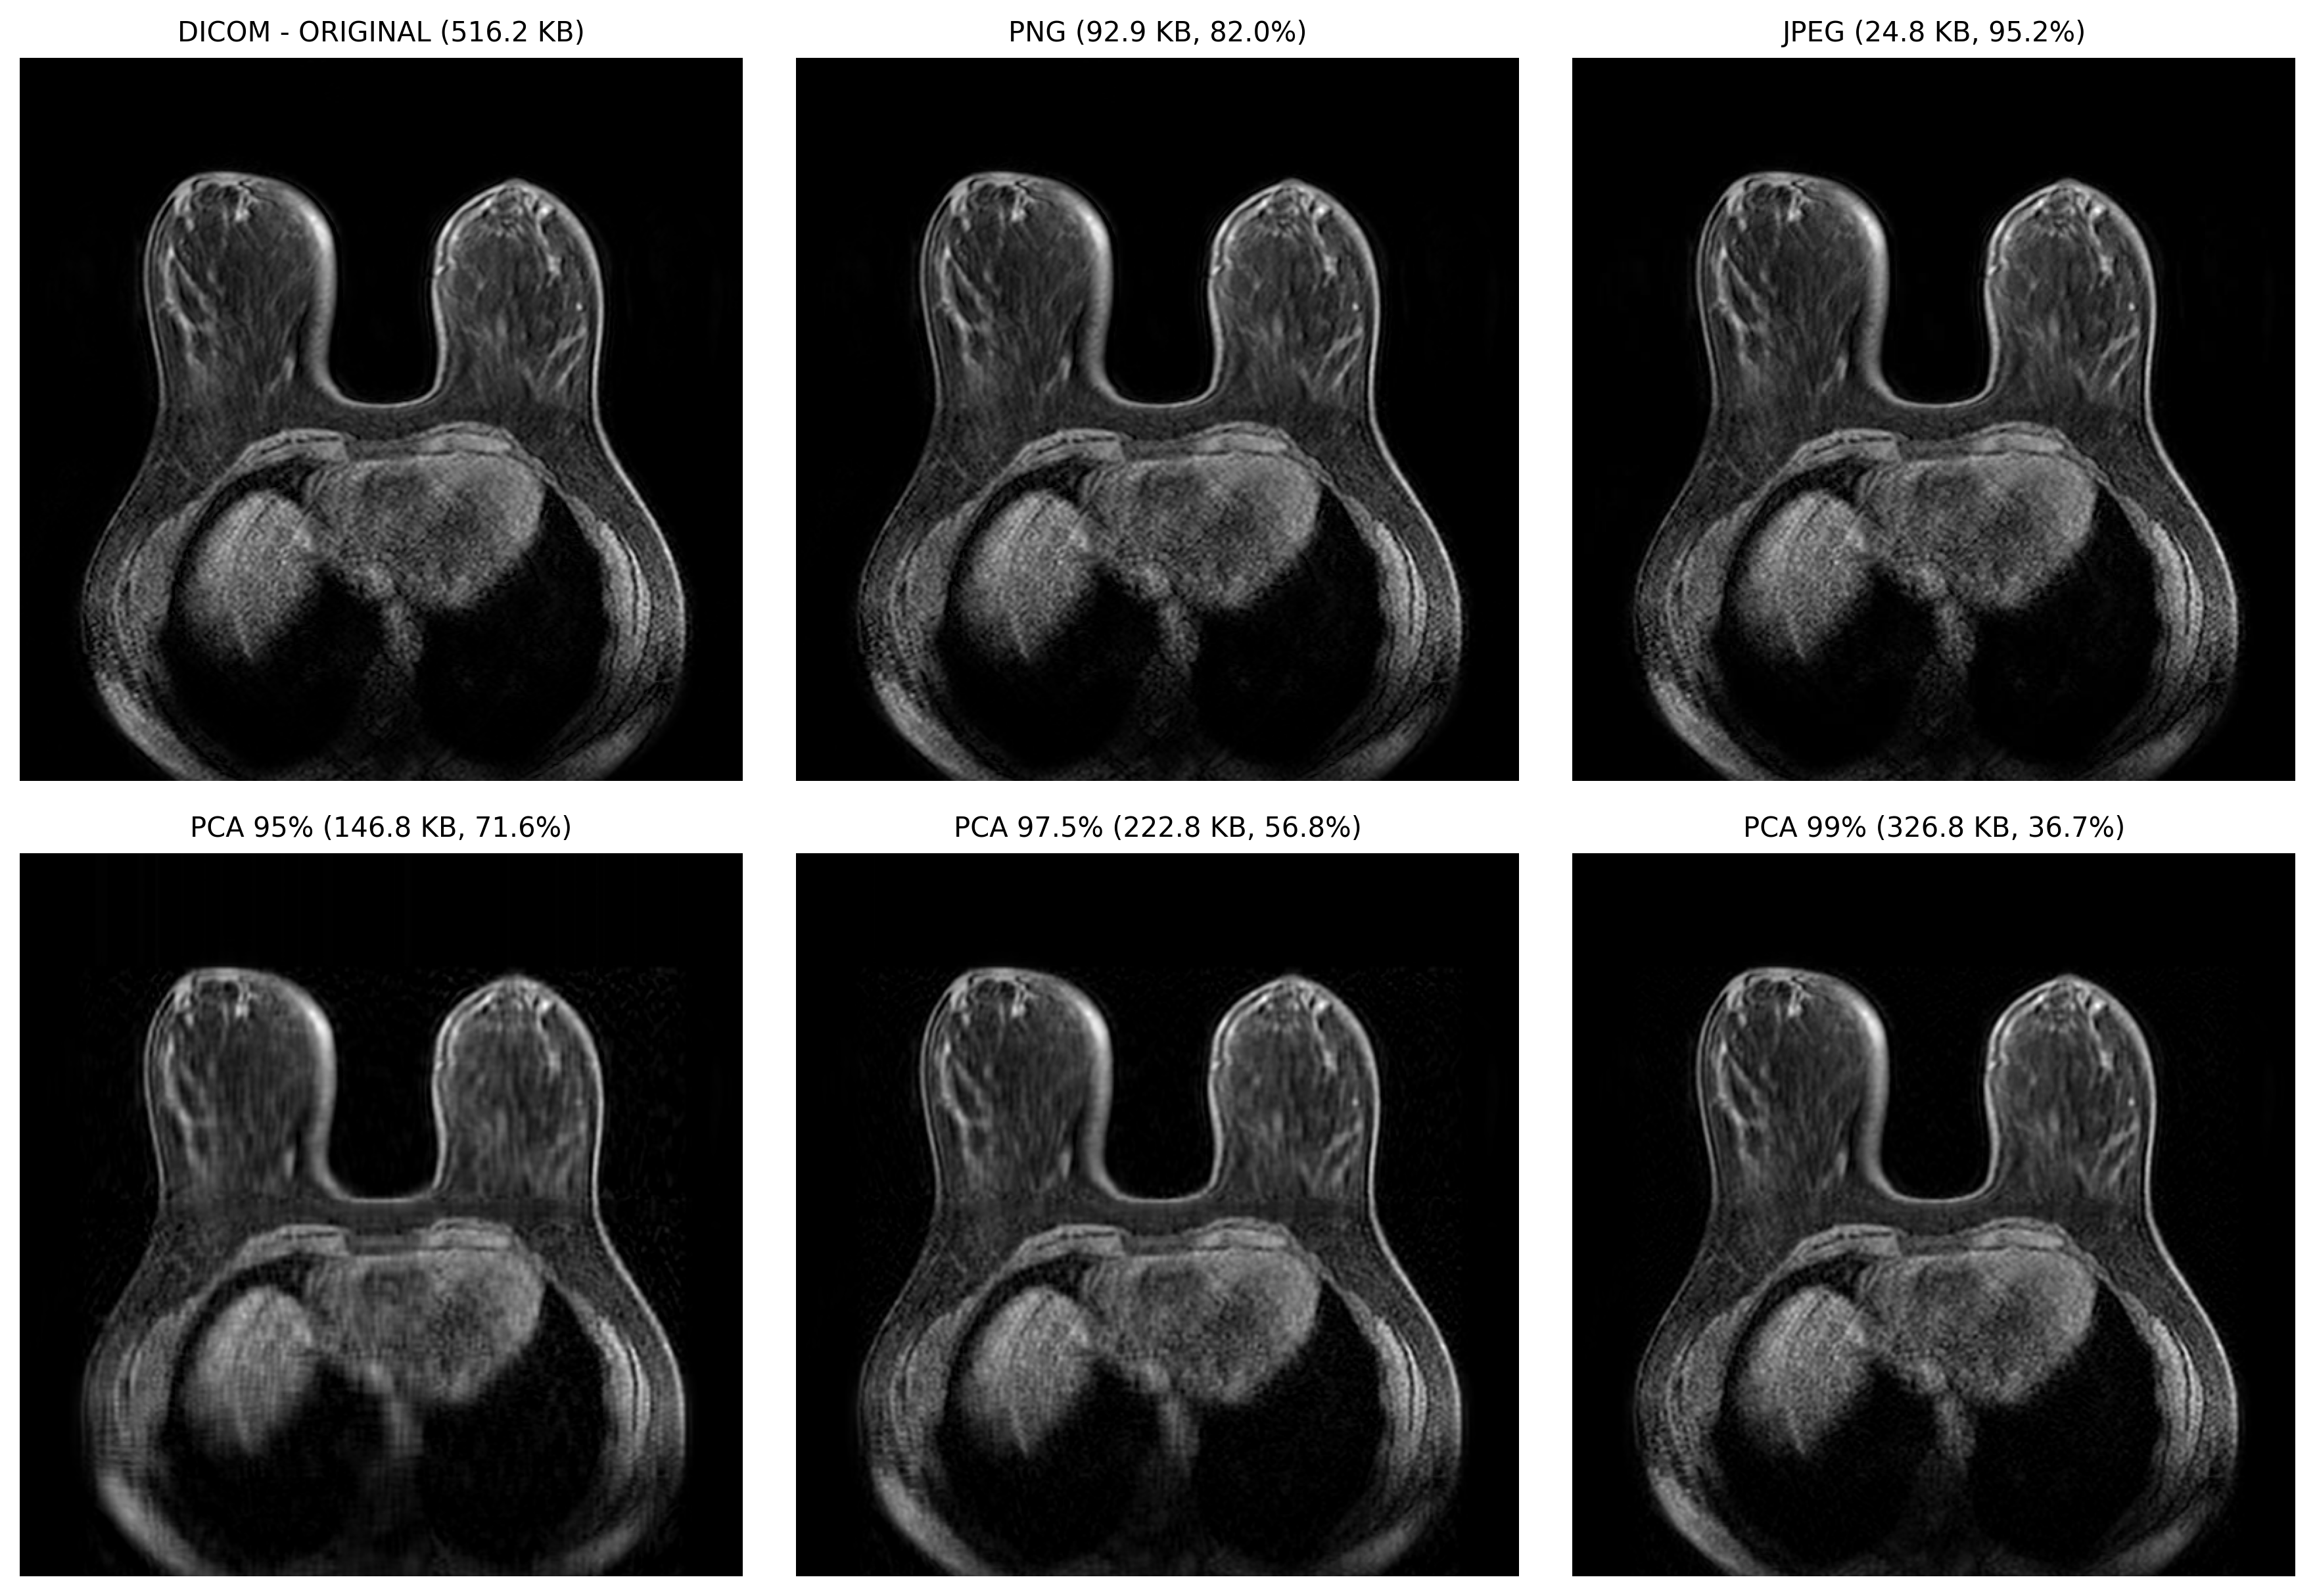
\includegraphics[width=\textwidth]{images/result-breast.png}
        }{
            \Fonte{Elaborado pelo autor.}
        }	
    \end{figure}
    \item \textbf{Cérebro:} Na Figura~\ref{fig:comparacao_cerebro}, observa-se as imagens de cérebro, que possuem uma combinação equilibrada entre áreas homogêneas e detalhadas. Essa característica resultou em compressões intermediárias, com perdas visuais moderadas dependendo do método e dos parâmetros utilizados, como observado no \acrshort{PCA}.
    \begin{figure}[H]
        \centering
        \UNIFORfig{
            \Caption{\label{fig:comparacao_cerebro} Comparação visual das imagens de cérebro: original e comprimidas por \acrshort{PNG}, \acrshort{JPEG} e \acrshort{PCA}.}
        }{
            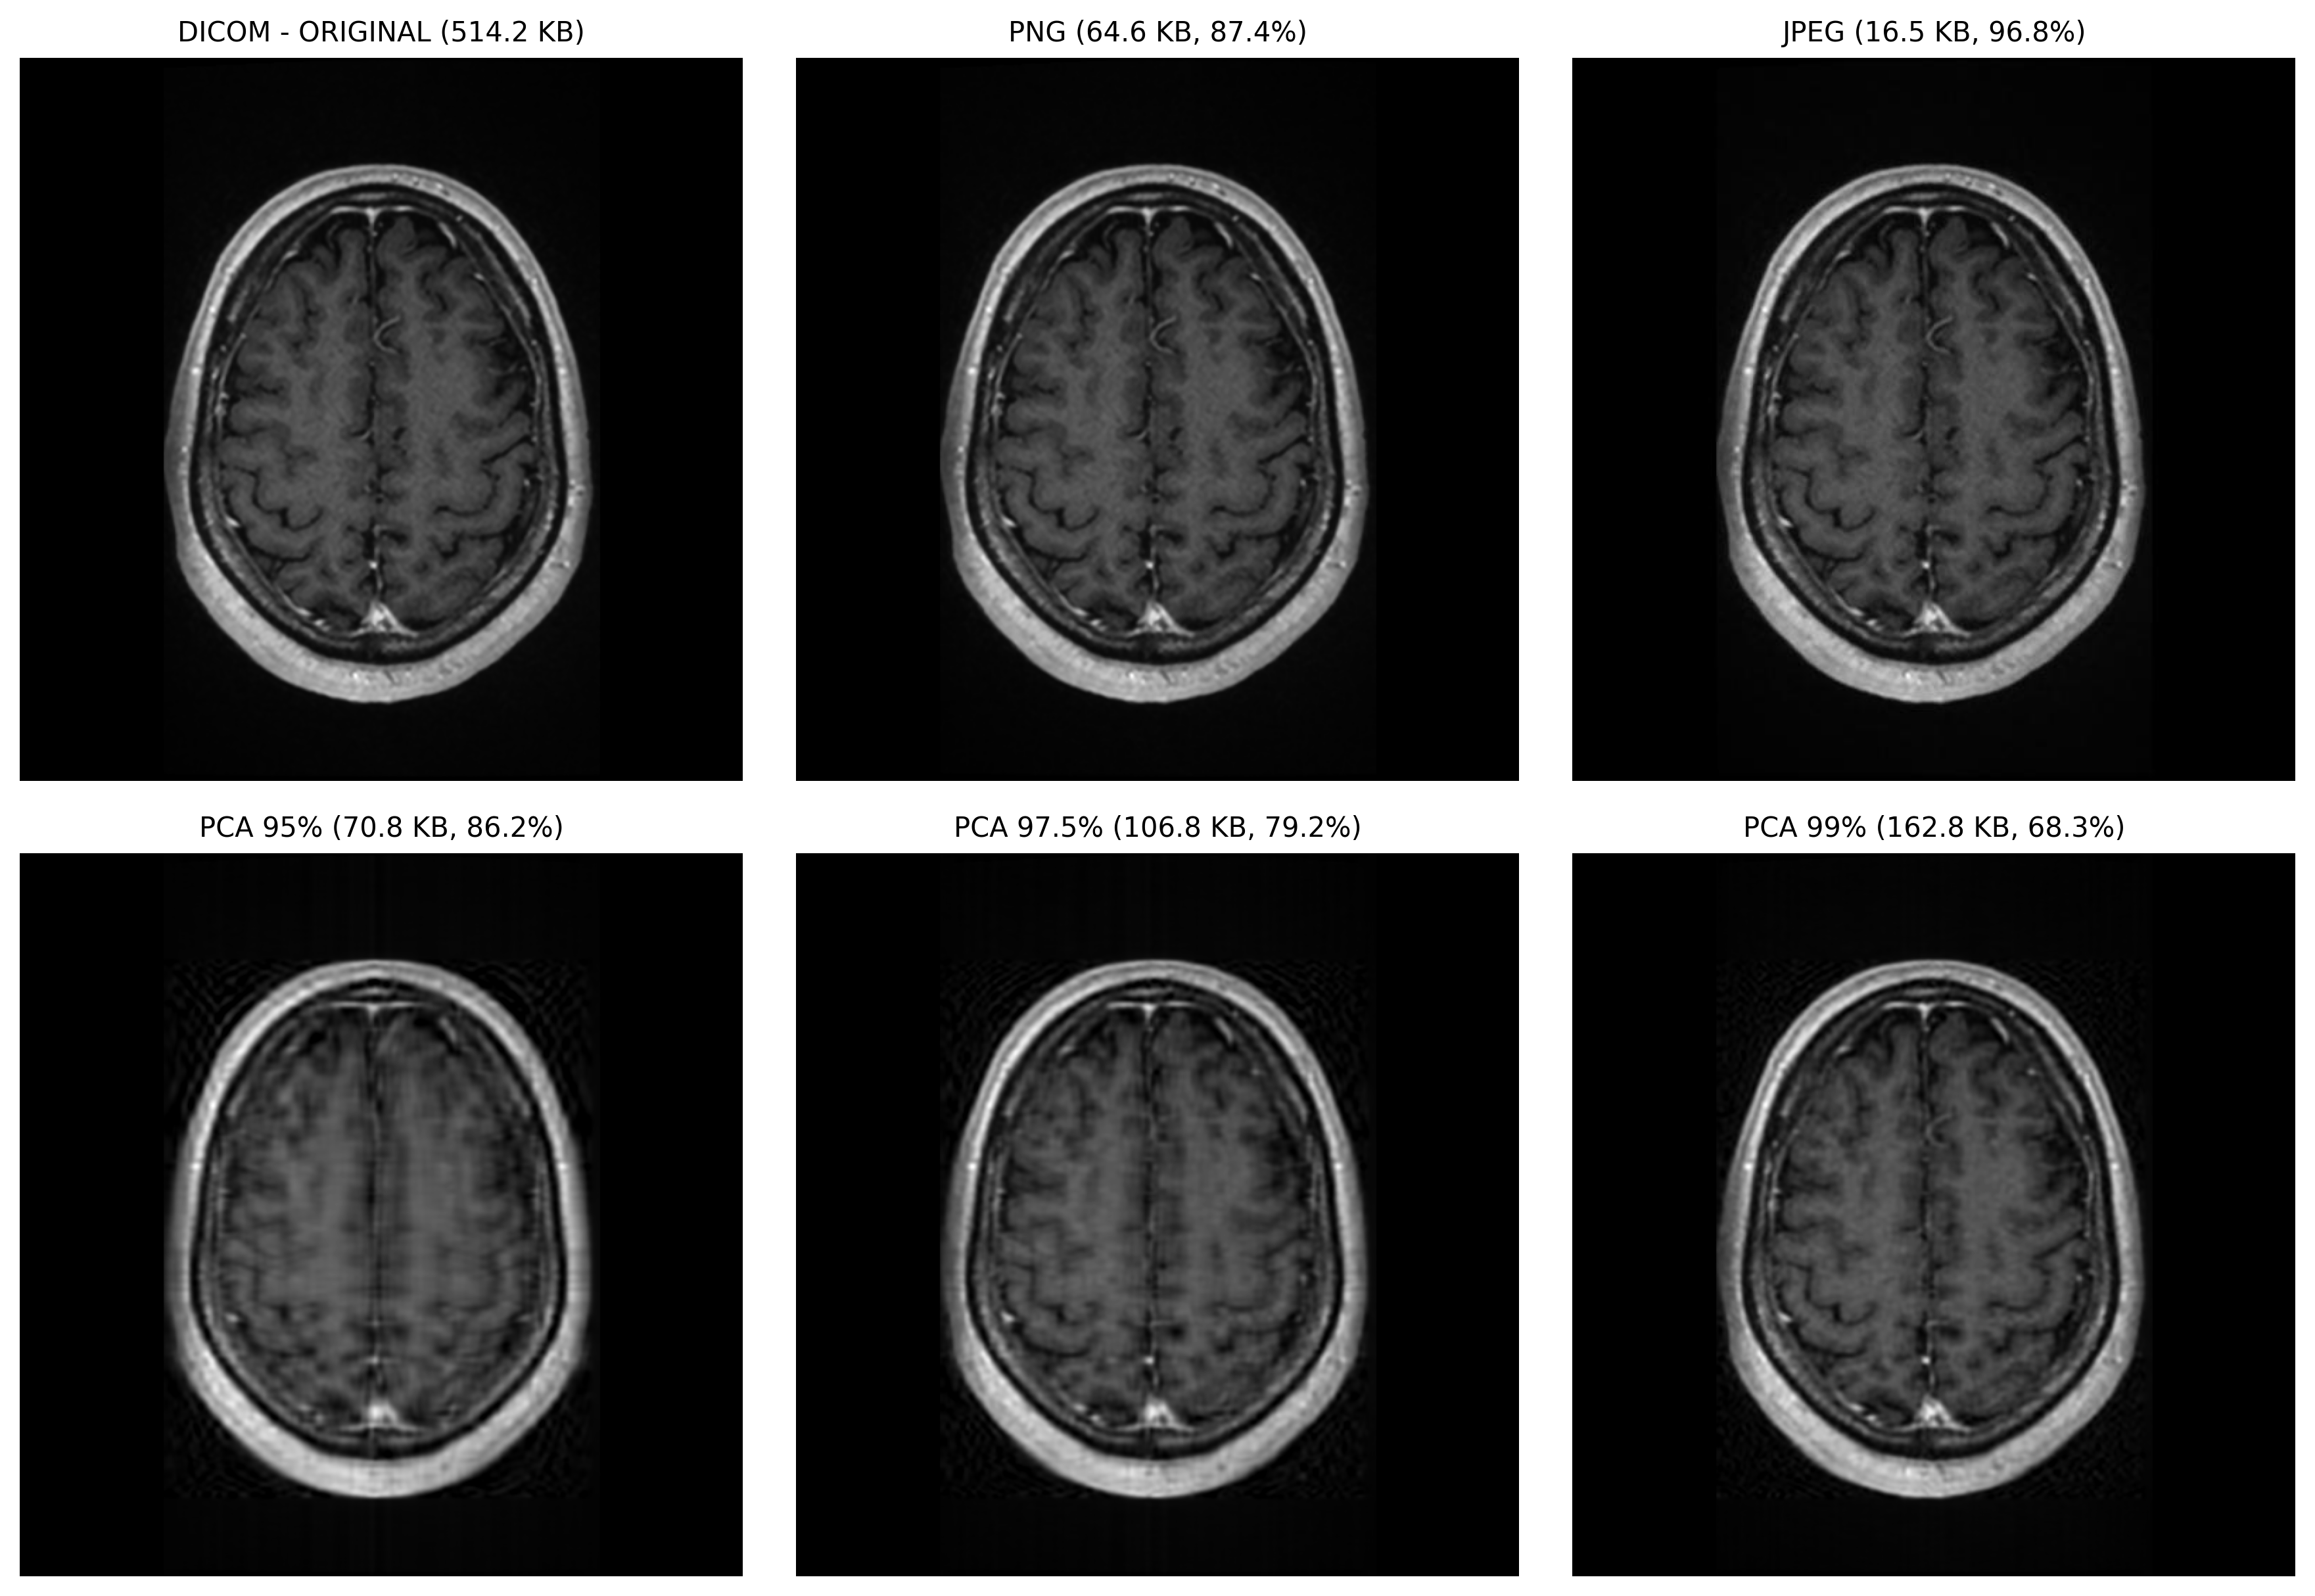
\includegraphics[width=\textwidth]{images/result-brain.png}
        }{
            \Fonte{Elaborado pelo autor.}
        }	
    \end{figure}
\end{itemize}

Estas figuras destacam que o método \acrshort{PNG} é ideal para preservação completa de qualidade, enquanto o \acrshort{JPEG} e o \acrshort{PCA} oferecem maior flexibilidade entre compressão e qualidade visual, dependendo dos parâmetros utilizados.

\section{Taxas de Compressão}

As taxas médias de compressão obtidas por cada algoritmo, agrupadas por tipo de órgão, estão apresentadas na Figura~\ref{fig:compression_by_algorithm_and_organ}. Observa-se que:

\begin{itemize}
    \item O algoritmo \textbf{\acrshort{JPEG}} alcançou as maiores taxas de compressão em todos os órgãos, superando 96\%.
    \item O \textbf{\acrshort{PNG}}, embora sem perdas, apresentou taxas de compressão em torno de 83-86\%, destacando-se pela capacidade de obter uma alta taxa de compressão mesmo sem ter perdas de informações.
    \item O \textbf{\acrshort{PCA}} teve desempenho variável conforme o percentual de variância explicada. À medida que a variância aumenta (de 95\% para 99\%), a taxa de compressão diminui, o que é esperado devido ao aumento na retenção de detalhes.
\end{itemize}

\begin{figure}[!htbp]
	\centering
	\UNIFORfig{
	    \Caption{\label{fig:compression_by_algorithm_and_organ} Taxas médias de compressão por tipo de órgão e método de compressão.}
	}{
	    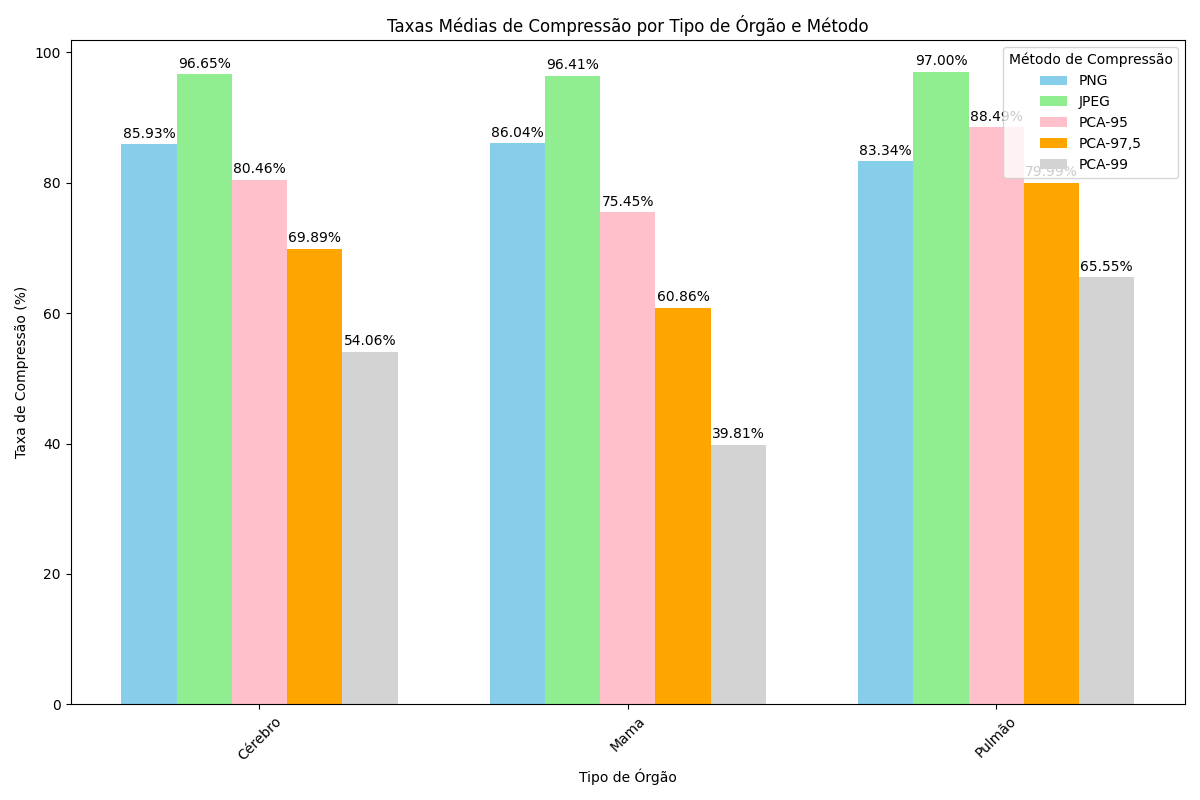
\includegraphics[width=\textwidth]{images/compression_by_algorithm_and_organ.png}
	}{
	    \Fonte{Elaborado pelo autor}
	}	
\end{figure}

\section{Taxas de Compressão por Método}

Para uma análise detalhada por algoritmo, foram gerados gráficos específicos para cada método, conforme apresentado a seguir:

\subsection{\acrshort{PNG}}

As taxas médias de compressão do \acrshort{PNG} estão ilustradas na Figura~\ref{fig:png_compression_by_organ}. O desempenho foi uniforme entre os órgãos, com taxas variando entre 83\% e 86\%.

\begin{figure}[H]
	\centering
	\UNIFORfig{
	    \Caption{\label{fig:png_compression_by_organ} Taxas médias de compressão \acrshort{PNG} por tipo de órgão.}
	}{
	    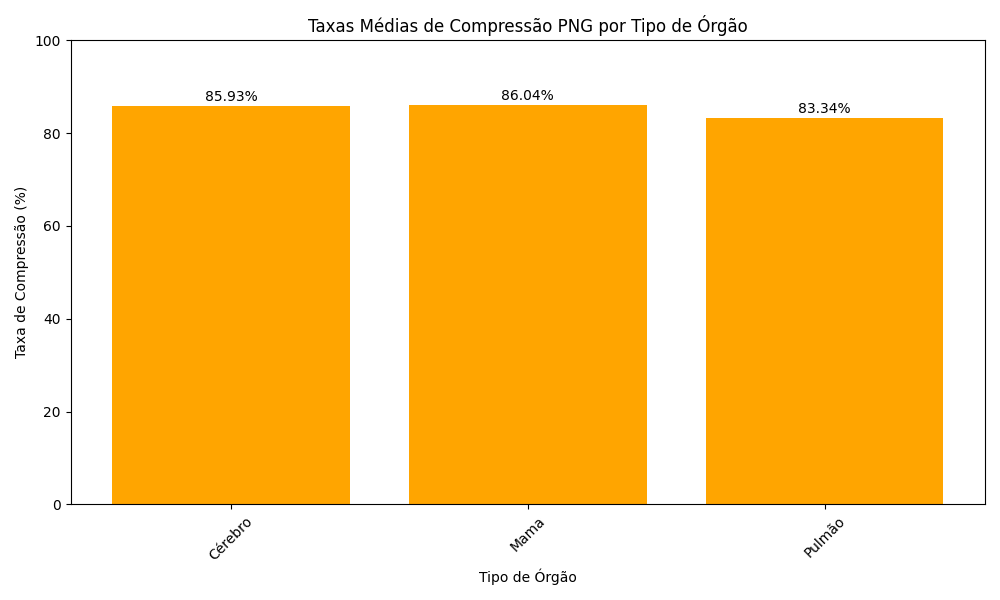
\includegraphics[width=0.8\textwidth]{images/png_compression_by_organ.png}
	}{
	    \Fonte{Elaborado pelo autor}
	}	
\end{figure}

\subsection{\acrshort{JPEG}}

A Figura~\ref{fig:jpeg_compression_by_organ} apresenta as taxas médias de compressão para o \acrshort{JPEG}. Este método apresentou as melhores taxas de compressão entre quase todos os algoritmos, alcançando valores superiores a 97\%.

\begin{figure}[H]
	\centering
	\UNIFORfig{
	    \Caption{\label{fig:jpeg_compression_by_organ} Taxas médias de compressão \acrshort{JPEG} por tipo de órgão.}
	}{
	    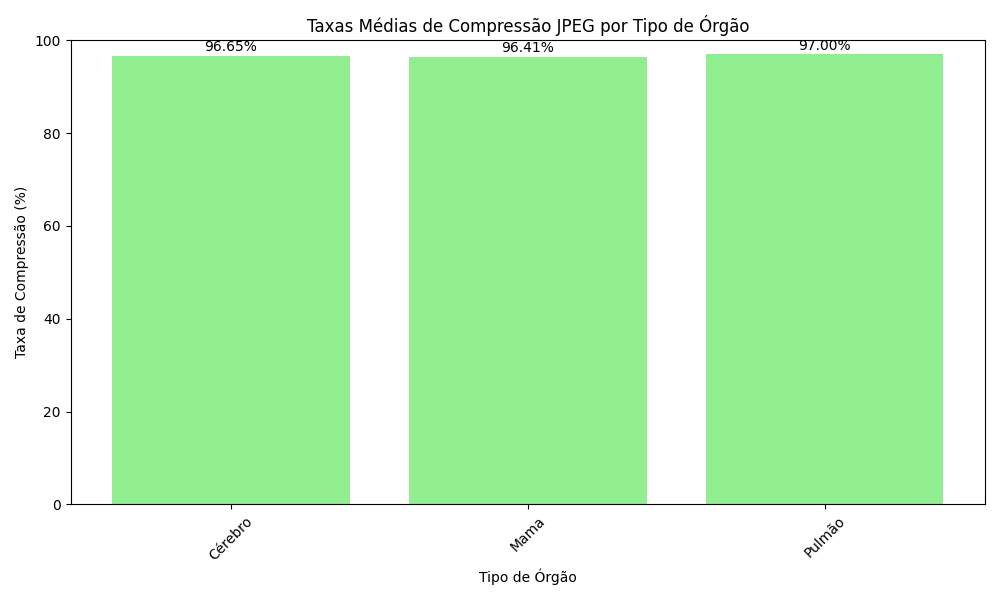
\includegraphics[width=0.8\textwidth]{images/jpeg_compression_by_organ.png}
	}{
	    \Fonte{Elaborado pelo autor}
	}	
\end{figure}

\subsection{\acrshort{PCA}}

As taxas médias de compressão para o \acrshort{PCA} são apresentadas nas Figuras~\ref{fig:pca-950}, \ref{fig:pca-975} e \ref{fig:pca-990}, referentes aos percentuais de variância explicada de 95\%, 97,5\% e 99\%, respectivamente. Observa-se que:

\begin{itemize}
    \item A compressão diminui à medida que aumenta o percentual de variância explicada, devido à retenção de mais detalhes.
    \item Órgãos com maior densidade de pixels (como pulmão) apresentam maior compressão, pois possuem mais áreas uniformes que facilitam a aplicação do \acrshort{PCA}.
\end{itemize}

\begin{figure}[H]
	\centering
	\UNIFORfig{
	    \Caption{\label{fig:pca-950} Taxas médias de compressão por tipo de órgão para o \acrshort{PCA} (95\% de variância explicada).}
	}{
	    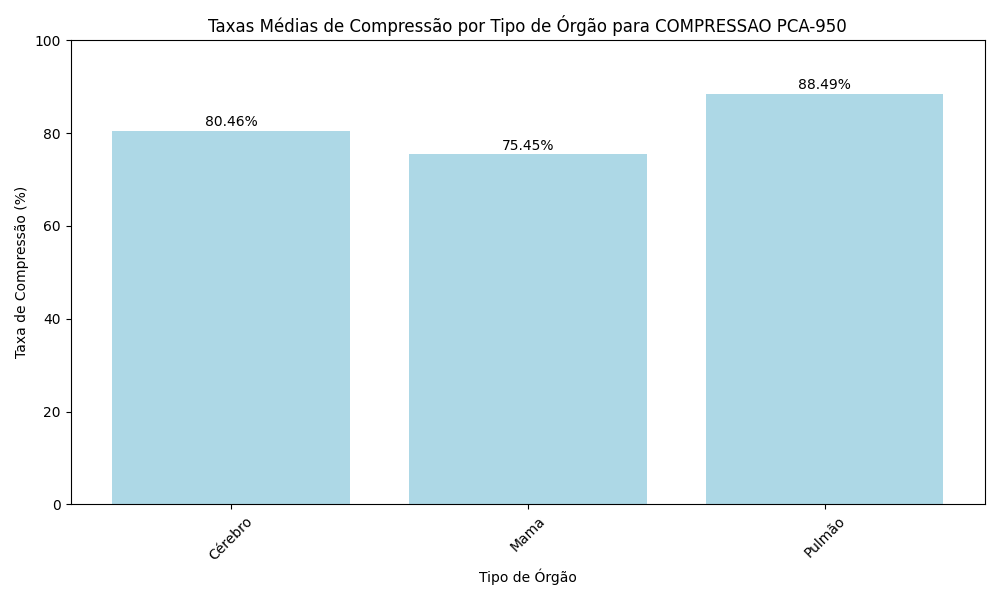
\includegraphics[width=0.8\textwidth]{images/pca-950_compression_by_organ.png}
	}{
	    \Fonte{Elaborado pelo autor}
	}	
\end{figure}

\begin{figure}[H]
	\centering
	\UNIFORfig{
	    \Caption{\label{fig:pca-975} Taxas médias de compressão por tipo de órgão para o \acrshort{PCA} (97,5\% de variância explicada).}
	}{
	    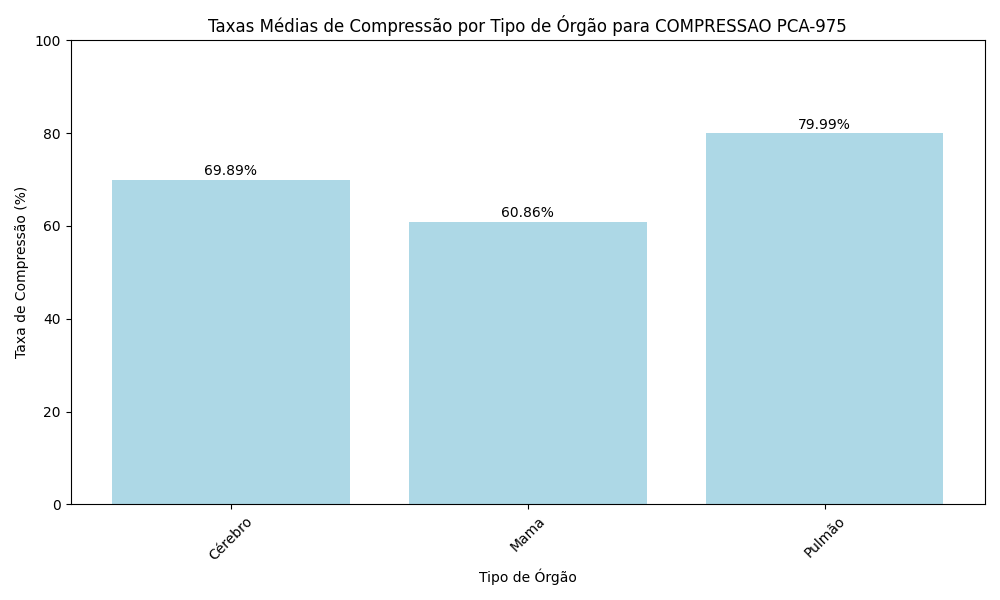
\includegraphics[width=0.8\textwidth]{images/pca-975_compression_by_organ.png}
	}{
	    \Fonte{Elaborado pelo autor}
	}	
\end{figure}

\begin{figure}[H]
	\centering
	\UNIFORfig{
	    \Caption{\label{fig:pca-990} Taxas médias de compressão por tipo de órgão para o \acrshort{PCA} (99\% de variância explicada).}
	}{
	    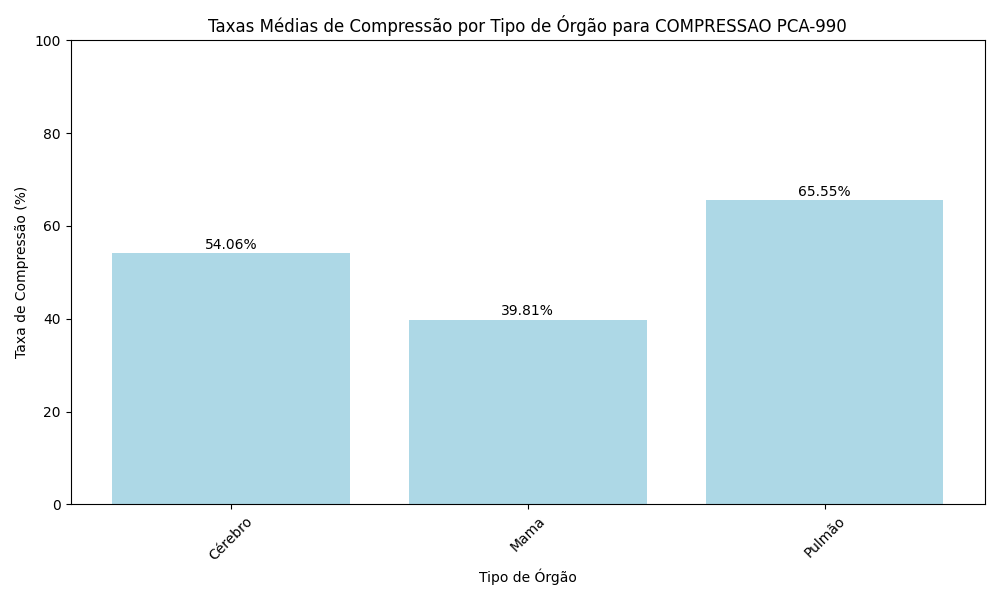
\includegraphics[width=0.8\textwidth]{images/pca-990_compression_by_organ.png}
	}{
	    \Fonte{Elaborado pelo autor}
	}	
\end{figure}

\section{Análise de Qualidade Aparente (\acrshort{PSNR})}

Os valores médios de \acrshort{PSNR} obtidos estão apresentados na Figura~\ref{fig:psnr_by_algorithm_and_organ}. Observa-se que:

\begin{itemize}
    \item O \textbf{\acrshort{PNG}} apresentou valores que tendem ao infinito, uma vez que é um método sem perda logo o \acrshort{MSE} resulta em 0, indicando qualidade visual idêntica à imagem original.
    \item O \textbf{\acrshort{JPEG}} manteve valores entre 42 e 45 dB, indicando uma alta qualidade, embora com perdas.
    \item O \textbf{\acrshort{PCA}} apresentou valores mais baixos para os percentuais de variância explicada de 95\% e 97,5\%, enquanto o PCA-99\% manteve valores próximos a 40 dB, destacando-se pela retenção de maior qualidade visual.
\end{itemize}

\begin{figure}[!htbp]
	\centering
	\UNIFORfig{
	    \Caption{\label{fig:psnr_by_algorithm_and_organ} Valores médios de \acrshort{PSNR} por algoritmo e tipo de órgão.}
	}{
	    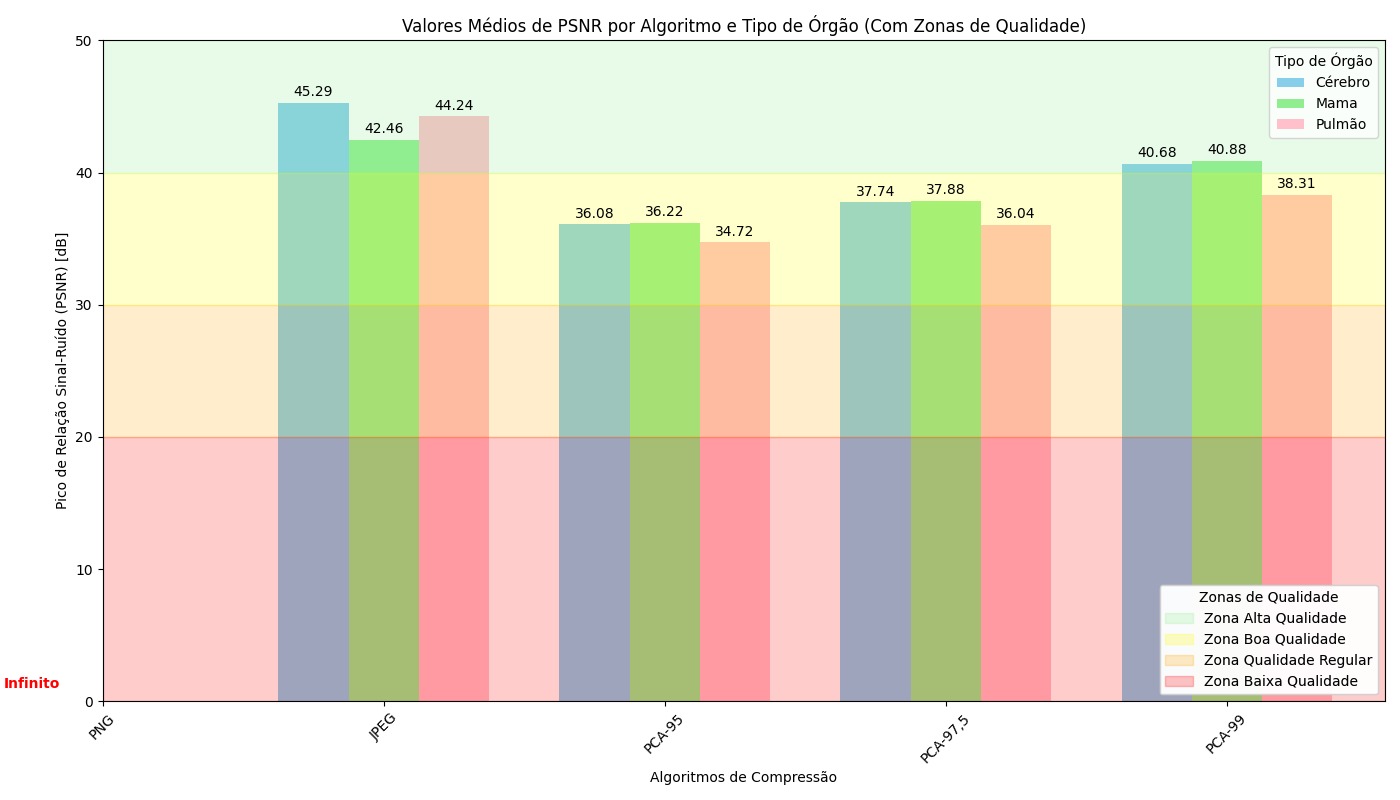
\includegraphics[width=\textwidth]{images/psnr_by_algorithm_and_organ.png}
	}{
	    \Fonte{Elaborado pelo autor}
	}	
\end{figure}

\section{Discussão dos Resultados}

Os resultados obtidos indicam que a escolha do algoritmo de compressão depende do objetivo:

\begin{itemize}
    \item O \textbf{\acrshort{PNG}} preserva integralmente a qualidade visual da imagem original, sendo indicado para casos onde a preservação completa da qualidade é imprescindível, como em aplicações críticas para diagnóstico médico. Este resultado é esperado, dado que o \acrshort{PNG} é um método de compressão sem perda, apresentando taxas de compressão consistentes e eficiência em manter a integridade das informações.
    \item O \textbf{\acrshort{JPEG}} é ideal para maximizar a compressão, mesmo com uma pequena perda de qualidade visual. Este método apresenta pequenas perdas de detalhes em áreas com maior densidade de informação (ex.: bordas e transições), mas as diferenças visuais são mínimas, tornando-o adequado para armazenamento de longo prazo e situações onde a redução significativa de tamanho é prioritária. 
    \item O \textbf{\acrshort{PCA}} oferece flexibilidade, permitindo ajustar o nível de compressão com base na variância explicada. No entanto, as diferenças visuais aumentam conforme o nível de variância explicada diminui, sendo que imagens comprimidas com 95\% de variância apresentam degradação visível em áreas de maior contraste. Em contrapartida, versões com 99\% de variância preservam melhor os detalhes visuais, ainda que com menor taxa de compressão. Esse método também requer maior processamento para reconstruir as imagens, o que deve ser considerado em contextos práticos.
\end{itemize}

A variação entre os órgãos pode ser atribuída às características específicas das imagens:

\begin{itemize}
    \item O \textbf{pulmão}, caracterizado por grandes áreas homogêneas devido à presença de espaços vazios (pretos) nas imagens de tomografia, favoreceu a compressão eficiente em todos os algoritmos. Essa característica reduz a complexidade da imagem, permitindo que métodos como o \acrshort{PCA} e o \acrshort{JPEG} explorem a redundância dos dados para alcançar altas taxas de compressão sem comprometer significativamente a qualidade visual.
    \item A \textbf{mama}, devido à sua alta densidade de detalhes e à textura mais heterogênea distribuída por toda a imagem, apresentou maior dificuldade para compressão. Essa complexidade aumenta a quantidade de informação que precisa ser mantida, especialmente para métodos como o \acrshort{PCA}, que depende de uma separação clara entre componentes principais e ruído. Como resultado, as taxas de compressão foram menores e as perdas de qualidade mais perceptíveis.
    \item O \textbf{cérebro}, com características intermediárias, combina áreas homogêneas, como o fundo da imagem, com regiões mais detalhadas, como o córtex cerebral. Essa composição balanceada permitiu que os algoritmos alcançassem resultados intermediários tanto em taxas de compressão quanto em qualidade visual. Enquanto o fundo homogêneo facilita a compressão, as regiões detalhadas impõem desafios que moderam o desempenho global dos algoritmos.
\end{itemize}

Esses resultados contribuem para a definição de estratégias eficientes de compressão em ambientes hospitalares, levando em consideração as características específicas das imagens médicas de cada órgão.
